\section{VideoGPT}
\label{sec:videogpt}

\begin{figure}
    \centering
    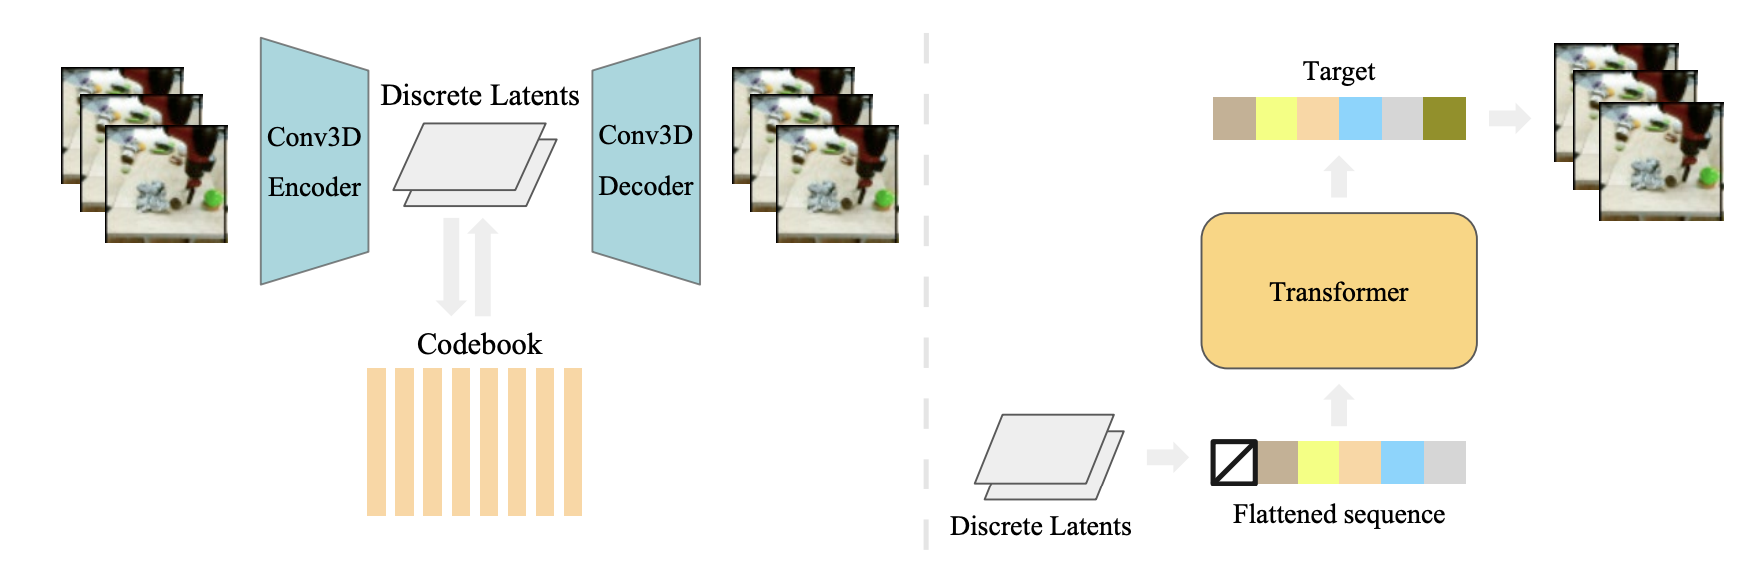
\includegraphics[width=0.7\textwidth]{images/video_gpt/architecture.png}
    \caption{VideoGPT architecture. Left: training the VQ-VAE; Right: training the autoregressive transformer model on the latent vectors.}
    \label{fig:videogpt_architecture}
\end{figure}

VideoGPT \cite{videogpt} uses likelihood based model VQ-VAE and GPT-like transformer model. The encoder of VQ-VAE first downsamples video into discrete latent space using 3D convolutions, and the decoder then reconstructs the video from these latent codes (by using a codebook - see VQ-VAE section \ref{vqvae}). The generated latents are decoded to the original video resolution as the training dataset.

The researchers take inspiration from image and video codecs: JPEG and MPEG for image and video compression. They contain the same spatio-temporal data as the uncompressed video, yet take less resources (by not working in the pixel space).

\subsection*{The VQ-VAE}

Reminder that the loss function of VQ-VAE is defined:

\begin{equation*}
    \mathcal{L} = \underbrace{\left| \left| x - D(e) \right| \right|^2_2}_{\mathcal{L}_\text{recon}} + \underbrace{\left| \left| \text{sg}\left[ E(x) \right] - e \right| \right|^2_2}_{\mathcal{L}_\text{codebook}} + \underbrace{\beta \left| \left| \text{sg}[e] - E(x) \right| \right|^2_2}_{\mathcal{L}_\text{commit}}
\end{equation*}

where $\text{sg}$ refers to stop-gradient, $\mathcal{L}_\text{recon}$ is the \textbf{reconstruction loss} (encourages the VQ-VAE to learn good representations to accurately reconstruct the data), $\mathcal{L}_\text{codebook}$ is the \textbf{codebook loss} (quantization loss, it brings codebook vectors closer to the encoder outputs), and $\mathcal{L}_\text{commit}$ is the \textbf{commitment loss} (which prevents the encoder outputs from fluctuating between different code vectors). 

The reconstruction loss optimizes only the decoder, the commitment loss optimizes only the encoder, and the codebook loss optimizes the codebook embeddings only. See section \ref{vqvae} for more details.

The researchers used EMA (exponential moving average which is described in the VQ-VAE paper \cite{vqvae}) update for the codebook loss. In short, it makes the VQ-VAE faster to train and converge.

\begin{figure}
    \centering
    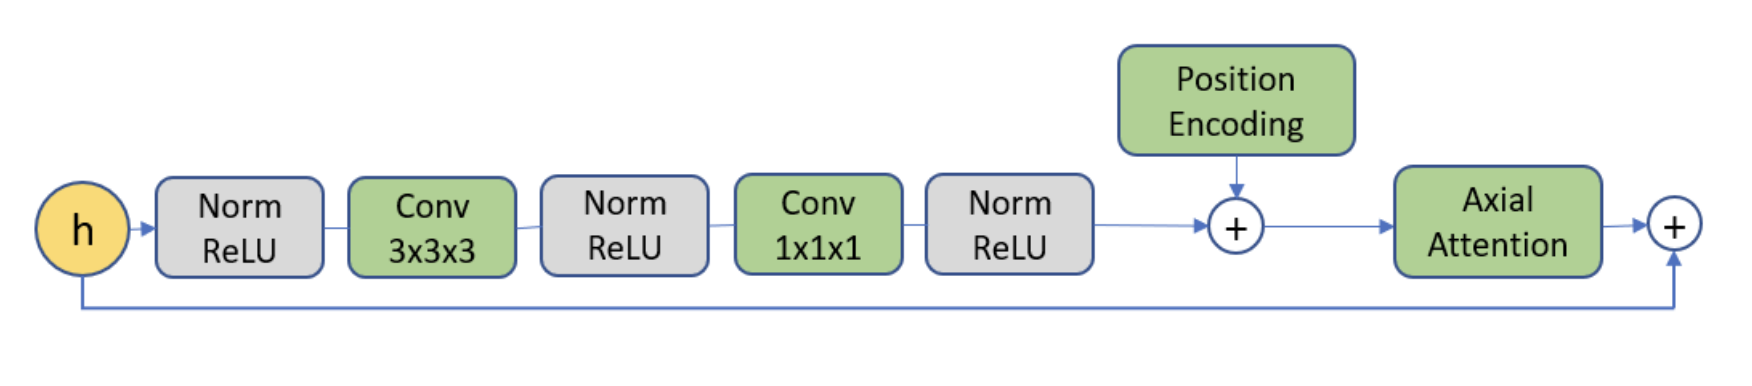
\includegraphics[width=0.75\textwidth]{images/video_gpt/res_atten_block.png}
    \caption{Residual attention block as described in VideoGPT. This block is used in the VQ-VAE model. The "Norm" layers are \texttt{LayerNorm} blocks (described in appendix \ref{appendix:blocks_norm}). The position embeddings is not explained in the paper; but we can infer them as the frame position (i.e. frame 0, 1, ... in the video), which is added element-wise.}
    \label{fig:videogpt_res_atten_block}
\end{figure}

To train the VQ-VAE model (to learn the latent codes), the authors trained the VQ-VAE on video data. The encoder consists of downsample 3D convolutions (appendix \ref{appendix:blocks_3dconv}) followed by attention residual blocks (figure \ref{fig:videogpt_res_atten_block}), and they used \texttt{LayerNorm}.

The architecture of the \textbf{decoder} is the reverse of the encoder (residual attention blocks followed by upscale 3D convolutions).

\subsection*{The transformer (GPT)}

As described in section \ref{sec:vq_gan}, GPT is autoregressive transformer model. The autoregressive nature can be described as $p(x) = \prod_{i=1}^{d} p(x_i | x_{\leq i})$ through masked self-attention. The GPT transformer is optimized through maximum likelihood (appendix \ref{appendix:likelihood_function}). The transformer follows the same prior networks as Image-GPT \cite{imagegpt}.

In \textbf{Image-GPT} the network learns to predict pixels and only a transformer is used, which is the first time a transformer-only image synthesis model was proposed (no CNN prior!). Instead of learning to predict tokens, the model learns to predict pixels. The network learns to predict the pixel values based on a probability distribution modeled on each of the previous pixels. The attention mechanism can map global spatial relationships, which helps in the modeling of the pixel distribution. The iGPT-XL model consists of 6.8 billion parameters, iGPT-M has 455 million parameters, and iGPT-S has 76 million parameters. 

In particular, the researchers wanted to test how generative pre-training can be useful to learn image representations in large scale.






\subsection{Architecture}

The architecture of VideoGPT is shown in figure \ref{fig:videogpt_architecture}.

\textbf{VQ-VAE:} They train the VQ-VAE on video data to learn the codebook. The encoder and decoder consists of 3D convolutions (appendix \ref{appendix:blocks_3dconv}) followed by attention residual blocks (figure \ref{fig:videogpt_res_atten_block}). Axial attention \cite{axial_attention} block is described in appendix \ref{appendix:attention}. The purpose of the VQ-VAE is to encode the video into discrete latent space. The purpose of the transformer is to autoregressively generate the video from these latents.

\textbf{Transformer:} The right side of figure \ref{fig:videogpt_architecture} shows the training of the autoregressive transformer model on the latent vectors. \textbf{The target is the next latent code (frame) in the video}. So the transformer learns to predict the next frame as a latent code (which is flatten vector, sequence).




\subsection{Video generation}

\begin{figure}
    \centering
    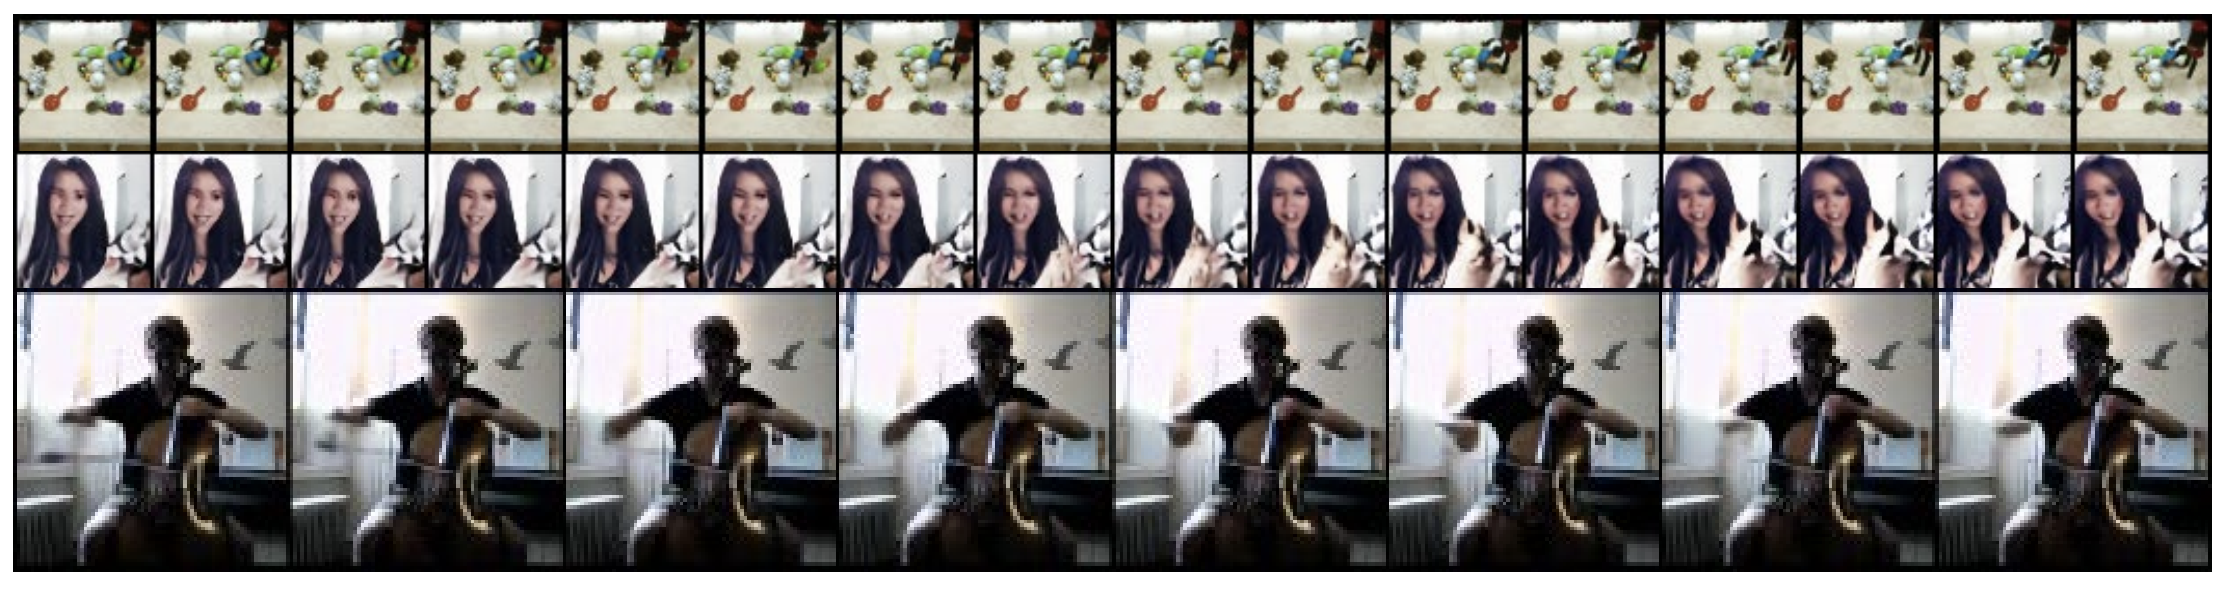
\includegraphics[width=0.8\textwidth]{images/video_gpt/video_generation.png}
    \caption{Video generation process in VideoGPT. The VQ-VAE encodes the video into discrete latents, and the transformer autoregressively generates the video from these latents.}
    \label{fig:videogpt_video_generation}
\end{figure}

The model can start to autoregressively generate videos given starting image: the VQ-VAE turns the first image to latent vector, and this vector is then fed to the GPT transformer to generate the next frame. The process is repeated until the desired number of frames is generated.

Multiple video generation examples are shown in figure \ref{fig:videogpt_video_generation}.